\documentclass{article}
\usepackage{graphicx}
\graphicspath{ {./} }

\title{ElasticSearch and Zipf’s and Heaps’ laws}
\date{Quadrimestre Tardor 2019 - 2020}
\author {
  Pol Renau Larrod\'e \\
  Felipe
}

\begin{document}
  \maketitle
  \newpage

  \section{Ley de Zipf}
  \paragraph{
  Nuestro objetivo en este apartado de la practica, es ver si una distribuci\'on de rango-frecuencia de las palabras en un gran corpus de datos, sigue la ley de la potencia.
  \\
  Con lo que tendremos que ver si  ajustando los par\'ametros de la siguiente funci\'on, encontramos una que describa a los datos, o se asemeje.
  \\
  \[ f = \frac{c}{(rank+b)^a} \]
  }
  \paragraph{
  Hemos realizado el análisis de datos sobre la colecci\'on de \textit{"corpus novels"} ya que a nuestro parecer eran los datos mas limpios.
  Indexamos todo el corpus de textos para extraer todas las palabras y sus respectivas frecuencias, usando el siguiente comando:
  \\
  \\
  \textit{ \$ python IndexFiles.py --index nov --path /path/to/novels}
  \\
  \\
  Una vez indexado el texto limpiamos el fichero de salida, eliminando urls, fechas, palabras que contengan n\'umeros dentro o que tengan s\'imbolos no admitidos en el lenguaje.
  De esta manera tenemos una entrada limpia con la que podemos empezar a trabajar.
  }
  \paragraph{
  Realizaremos la experimentaci\'on con las 10000 palabras con la frecuencia más alta. Fijamos valores para la \textit{a}, y usamos la funci\'on de \textit{curve fit} para encontrar los valores \'optimos para b i c.
Empezamos con 0.5, no obstante con este valor la grafica de los datos quedaba bastante por debajo que la de "fitting" ,
   as\'i que modificamos el valor de \textit{a} hasta 1.05, en este punto encontramos que la curva de "fitting" es muy parecida a la de datos.     }
\newpage

 \begin{figure}[!tbp]
   \begin{minipage}[b]{0.4\textwidth}
     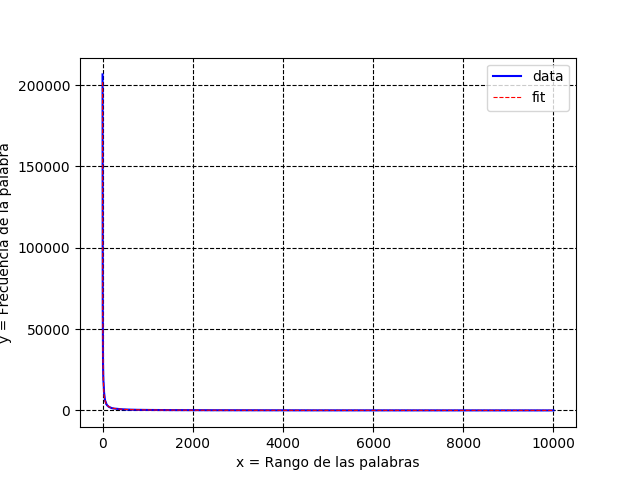
\includegraphics[width=\textwidth]{novels}
   \end{minipage}
   \hfill
   \begin{minipage}[b]{0.4\textwidth}
     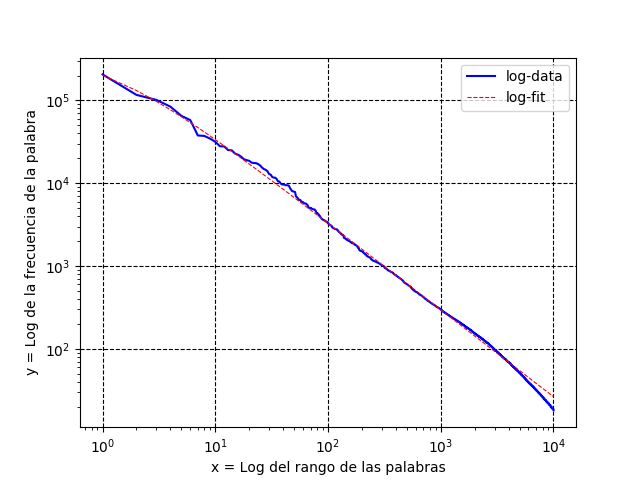
\includegraphics[width=\textwidth]{novels-Log-Log}
   \end{minipage}
 \end{figure}
 \paragraph{
 Finalmente vemos que los datos siguen la tendencia de la ley de potencia.
 Y que entonces la ley de Zipf tiene seg\'un nuestros datos una tendencia de:
 \\
 \[ f(x) = \frac{417936}{(x+1.007)^{1.05}} \]
 }
\newpage
  \section{Ley de Heap}


\end{document}
